
                \begin{figure}
                    \centering
                    \begin{tikzpicture}
                        \pgfplotsset{%
                            width=1\textwidth,
                            height=0.4\textheight
                        }
                        \begin{axis}[
                            xlabel={Start temperature},
                            ylabel={Average dynamic energy (watt)},
                            ymin=0,ymax=100,
                        ]
                        
                            \addplot [mark=none, densely dashed, red]  coordinates {
                            (35, 43.79567025634117)(40, 41.33243335734464)(45, 39.79192119250021)
                            };
                            \addlegendentry{WRK - IPG}
                            
                            \addplot [mark=none, densely dashed, blue]  coordinates {
                            (40, 41.35209258186638)(45, 40.41048085252703)(60, 41.4877758236443)
                            };
                            \addlegendentry{WRK - LHM}
                            
                            \addplot [mark=none, densely dashed, cyan]  coordinates {
                            (40, 32.64789590191951)(45, 33.5055623395402)(50, 35.29689520397377)
                            };
                            \addlegendentry{WRK - CLAMP (win)}
                            
                        \end{axis}
                    \end{tikzpicture} 
                \caption{A graph illustrating the energy consumption of Cores for test case FannkuchRedux with regards to the temperature of the DUT, experiment \#2, (with outliers)} \label{fig:FannkuchRedux_Cores_temperature_exp2}
                \end{figure}
                